\documentclass{beamer}

%\usepackage{subfigure}
\usepackage{graphicx}
\usepackage{sidecap}
\usepackage{caption}
\usepackage{subcaption}
\captionsetup{compatibility=false}
\usepackage{appendixnumberbeamer}
\usepackage{amsmath}
% --
\usepackage{multirow}
\usepackage{xcolor}
\usepackage{setspace}
\usepackage{hyperref}
\usepackage{anyfontsize}

\setbeamertemplate{footline}

\newenvironment{itemise} {\begin{itemize} \setlength{\itemsep}{0.2cm}} {\end{itemize}}
\usepackage[labelformat=empty]{caption}
\setbeamertemplate{sections/subsections in toc}[square]

%% COLORS
\definecolor{Gray}{gray}{0.9}
\definecolor{dblue}{rgb}{0.132,0.1,0.27}
\definecolor{mint}{cmyk}{1.0, 0.2, 0.6, 0.05}
\definecolor{ant}{cmyk}{0.5, 0.1, 0.0, 0.45}
\definecolor{lgray}{cmyk}{0.12, 0.0, 0.0, 0.17}
\definecolor{lred}{cmyk}{0.0, 0.9, 0.7, 0.0}


\usepackage{etoolbox}% http://ctan.org/pkg/etoolbox 
\usepackage{booktabs}

\newenvironment{literatur}{%
  \parskip2pt \parindent0pt \raggedright
  \def\lititem{\hangindent=0.5cm \hangafter1}}{%
  \par\ignorespaces}

\newcommand{\tb}[1]{{\color{blue}{\textbf{#1}}}}
\newcommand{\tm}[1]{{\color{mint}{\textbf{#1}}}}
\newcommand{\tr}[1]{{\color{red}{\textbf{#1}}}}
% Ilya: packages

\usepackage{tikz}
\usepackage{lmodern}
\usepackage{enumitem}

% Ilya: my commands

\newenvironment{mytemize}
{\vfill\itemize[nolistsep,itemsep=\fill,label=\color{blue}{$\triangleright$}]}
  {\enditemize}


\newenvironment{mynumerate}
{\vfill\enumerate[nolistsep,itemsep=\fill,label=\arabic*.]}
  {\endenumerate}

\newcommand{\hitem}[1]{
  {\color{blue}{$\triangleright$}} 
  {#1} 
  {\hfill}
}

\setlist[itemize]{label= \color{blue}{$\triangleright$}}
\setlist[enumerate]{label = \arabic*.}

\newcommand{\rarr}{$\Rightarrow$\ }

%------------------------------------------------------------------------------------
% TITLE
%------------------------------------------------------------------------------------
\title[PSME]{Macroeconomics\\ Lecture 8 -- New Keynesian Model}
\author[I. Eryzhenskiy]{Ilya Eryzhenskiy}
\institute[Paris-1]{PSME Panth\'{e}on-Sorbonne Master in Economics}
\date[PSME macro]{Fall 2022}

%---BEGIN------------------------------------------------------------------------------
\begin{document}
%---BEGIN------------------------------------------------------------------------------
\begin{frame}
\maketitle
\end{frame}
%---FRAME------------------------------------------------------------------------------
%\section{Outline}
\begin{frame}
\frametitle{Outline}
\tableofcontents
\end{frame}
%---FRAME------------------------------------------------------------------------------
%---FRAME------------------------------------------------------------------------------
%---FRAME-----------------------------------------------------------------------------
\begin{frame}{The basic New Keynesian model}

\begin{mytemize}
\small
\item Also uses the \tb{microfoundations} as in RBC framework
\begin{mytemize}
\small
\item rational expectations
\item representative, infinitely lived agents
\item optimizing behaviour 
\end{mytemize}
\item But \tr{important differences}
\begin{mytemize}
\small
\item a large number (continuum) of consumption goods 
\begin{mytemize}
\item[\rarr] not perfectly substitutable for HH \rarr no perfect competition $\rightarrow$ \tm{monopolistic competition}
\end{mytemize}
\item prices for goods not flexible $\rightarrow$ \tm{nominal rigidities}
\end{mytemize}
\item We will also make simplifications w.r.t. RBC:
no capital accumulation $\rightarrow$ production with labor only
\item Versions of this model widespread in central banks, commercial banks, public authorities, international organizations\dots
\end{mytemize}

\end{frame}
%---FRAME------------------------------------------------------------------------------
\begin{frame}{The basic New Keynesian model}

\begin{mytemize}
\small
\item \textbf{Households}
\begin{mytemize}
\small
\item consume \tb{a bundle of diversified goods} 
\item supply labour 
\item make saving in a \tb{nominal bond} (zero in equilibrium)
\end{mytemize}
\item \textbf{Firms}
\begin{mytemize}
\small
\item a continuum of firms of measure one
\item each \textbf{producing a single, imperfectly substitutable good}
\item only using labour as factor input 
\item pricing the good
\begin{mytemize}
\item under monopolistic competition 
\item given \tm{nominal rigidities} (but we start with a \tm{flexible price} version today)
\end{mytemize}
\end{mytemize}
\end{mytemize}

\end{frame}
%---FRAME------------------------------------------------------------------------------
\section{Household}
%---FRAME------------------------------------------------------------------------------
\begin{frame}
\frametitle{Outline}
\tableofcontents[currentsubsection]

\end{frame}
%---FRAME------------------------------------------------------------------------------
\begin{frame}{Household}
  Household utility has the form $E_0 \sum_{t=0}^{\infty} \beta^t U(C_t,L_t)$, and we will work with \textit{isoelastic} utility for both $C$ and $L$:
\begin{align*}
U(C_t,L_t) = \frac{C_t^{1-\sigma}}{1-\sigma} - \frac{L_t^{1-\eta}}{1-\eta}
\end{align*}
where $C_t$ is a \tb{consumption indicator} constructed with a large number of goods, each having index $i$. \\ $C_t$ calculated with \tb{aggregator function} proposed by Dixit and Stiglitz: 
\begin{align*}
C_t \equiv \left( \int_0^1 C_t(i)^{\frac{\varepsilon-1}{\varepsilon}} di\right)^{\frac{\varepsilon}{\varepsilon-1}},
\end{align*}
where $C_t(i)$ is the quantity of \alert{good $i$} consumed by the household. 
\\
\vfill
Each good has its own price $P_t(i)$ set by a firm producing the good.

\end{frame}
%---FRAME------------------------------------------------------------------------------
%\begin{frame}{Monopolistic competition}
%
%\begin{mytemize}
%\small
%\item HH must now decide how to allocate its consumption expenditures among different goods
%\item All goods are different and not perfect substitutes
%\item $\rightarrow$ \tm{monopolistic competition} following the Dixit-Stiglitz (AER 1977) model
%\begin{mytemize}
%\small
%\item most common specification of imperfect competition in macro models
%\item (near-) universal building block of modern sticky price models
%\item \tb{Idea:} {\textcolor{blue}{imperfectly-substitutable goods combined yield an aggregate good}}
%\end{mytemize}
%\end{mytemize}
%{
%\small
%\begin{align*}
%C_t \equiv \left( \sum_{i=1}^{N} C_{i,t}^{\frac{\alert{\varepsilon}-1}{\alert{\varepsilon}}} \right)^{\frac{\alert{\varepsilon}}{\alert{\varepsilon}-1}} & \quad \text{(discrete case)}\\
%C_t \equiv \left( \int_0^1 C_t(i)^{\frac{\alert{\varepsilon}-1}{\alert{\varepsilon}}} di\right)^{\frac{\alert{\varepsilon}}{\alert{\varepsilon}-1}} & \quad \text{(continuous case)}
%\end{align*}
%}
%\end{frame}
%---FRAME------------------------------------------------------------------------------
\begin{frame}{Differentiated goods}

\begin{mytemize}
\item imperfectly-substitutable goods combined yield an aggregate good
  \begin{mytemize}
  \item Sometimes assumed that intermediary firms combine the goods for the household \rarr the aggregator is their production function
  \end{mytemize}
\begin{align*}
%C_t \equiv \left( \sum_{i=1}^{N} C_{i,t}^{\frac{\alert{\varepsilon}-1}{\alert{\varepsilon}}} \right)^{\frac{\alert{\varepsilon}}{\alert{\varepsilon}-1}} & \quad \text{(discrete case)}\\
C_t \equiv \left( \int_0^1 C_t(i)^{\frac{\alert{\varepsilon}-1}{\alert{\varepsilon}}} di\right)^{\frac{\alert{\varepsilon}}{\alert{\varepsilon}-1}} %& \quad \text{(continous case)}
\end{align*}

\item $\varepsilon$ is the \tr{constant elasticity of substitution (CES)} between any pair of differentiated goods
\item \tb{Properties of the aggregator}
\begin{mytemize}
\item (1) symmetric, (2) strictly increasing, (3) strictly concave in all arguments, (4) homogeneous of degree one
\end{mytemize}
\end{mytemize}

\end{frame}
%---FRAME------------------------------------------------------------------------------
\begin{frame}{Household}

Households maximize the consumption index $C_t$ for any given level of expenditures $\zeta_t \equiv\int_0^1 P_t(i) C_t(i) di$. The solution yields a set of demand equations
\begin{align}
C_t(i) = \left(\frac{P_t(i)}{P_t}\right)^{-\varepsilon}C_t \quad \text{for all }i \in [0,1], \tag{1}
\end{align}
where $P_t \equiv [\int_0^1 P_t(i)^{1-\varepsilon}di]^{1/(1-\varepsilon)}$ is an aggregate price index. This allows to write total consumption expenditure as
\begin{align*}
\int_0^1 P_t(i) C_t(i) di = \alert{P_t C_t}
\end{align*}
\end{frame}
%---FRAME------------------------------------------------------------------------------

\begin{frame}{Household budget constraint}
The flow budget constraint is
\begin{align*}
  \int_0^1 P_t(i) C_t(i) di + B^N_{t+1} \leq (1+i_t)B^N_{t} + W^N_t L_t + \Pi^N_t 
\end{align*}
with $C_t(i)$ period $t$ consumption of good $i$, $P_t(i)$ price of good $i$, $L_t$ hours of work, $W^{\tr{N}}_t$ \tr{n}ominal (i.e. in units of currency) wage, $B^{\tr{N}}_t$~\tr{n}ominal value of bonds held at beginning of $t$, $i_t$ the nominal interest rate, $\Pi^{\tr{N}}_t$ \tr{n}ominal profits. 
%\\
%A transversality condition $lim_{T\rightarrow \infty}E_t[B^n_t]\geq0$ for all $t$ applies.
\\ \vfill
Using consumption aggregator and price indicator%$P_t \equiv [\int_0^1 P_t(i)^{1-\varepsilon}di]^{1/(1-\varepsilon)}$
, the constraint can be rewritten:
\begin{align*}
  P_t C_t + B^n_{t+1} \leq (1+i_t)B^n_{t} + W^n_t L_t + \Pi^n_t
\end{align*}

\end{frame}

%\begin{frame}{Household}
%
%\small
%\begin{mytemize}
%\small
%\item The budget constraint simplifies to
%\[
%P_t C_t + Q_t B_t \leq B_{t-1} + W_t L_t + T_t
%\]
%\item FOC of the household w.r.t. consumption and labour
%\begin{align*}
%\frac{-u_n(c_t,1-n_t)}{u_c(c_t,1-n_t)}&= \frac{W_t}{P_t} \\
%Q_t&=\beta E_t \left[ \frac{u_c(c_{t+1},1-n_{t+1})}{u_c(c_t,1-n_t)} \frac{P_t}{P_{t+1}}\right]
%\end{align*}
%\end{mytemize}
%
%\end{frame}
%---FRAME------------------------------------------------------------------------------
\begin{frame}{Households' optimization} 

Using same approach as in the RBC, we obtain the FOCs: 
\begin{align*}
\beta E_0 \left[ \frac{C_{t+1}^{-\sigma}}{C_t^{-\sigma}} \frac{P_t}{P_{t+1}}\right] = \frac{1}{1+i_{t+1}} \\
-\frac{L_t^{\eta}}{C_t^{\sigma}}= \frac{W^N_t}{P_t} 
\end{align*}
\vfill
We will use lowercase letters for logs of variables: $c_t = \ln C_t, l_t = \ln L_t$, etc.:
\begin{align*}
c_t &= E_t[c_{t+1}] -\frac{1}{\sigma} (i_t-E_t[\pi_{t+1}]-\rho)  \\
\sigma c_t + \eta l_t &= w^N_t - p_t  \\
%\text{with } &i_t \equiv -log Q_t \\
\text{with } \rho &= -\ln \beta \ \ \text{the discount \tr{rate} (used in continuous time models)}
\end{align*}

\end{frame}
%---FRAME------------------------------------------------------------------------------
%\begin{frame}{Excursion: Log-linearization}
%
%{
%\small
%\begin{mytemize}
%\item DSGE models lead to system of nonlinear difference equations
%\item We said that no analytical solution exists $\rightarrow$ approximation techniques
%\item One widely adopted approach is \tb{log-linearization}
%\begin{enumerate}
%\item \alert{Linear system} of difference equations can be solved (... and that is what the software dynare does, among other things)
%\item Taking logs helps to interpret the \alert{units as percentages} (in deviations from steady state)
%\end{enumerate}
%\item Cookbook procedure:
%\begin{enumerate}
%\item Take natural logarithm
%\item Make first-order Taylor series expansion (around steady state)
%\item Simplify so that variables have interpretation as percentage deviations
%\end{enumerate}
%\end{mytemize}
%}
%
%\end{frame}
%%---FRAME------------------------------------------------------------------------------
%\begin{frame}{Excursion}
%
%{
%\small
%\tb{Log-linearization}
%\begin{mytemize}
%\item Assume a function $f(x)= g(x)/h(x)$
%\item Then, a log-linear approximation would include taking the natural logarithm on both sides, ln$f(x)=$ ln$g(x)$-ln$h(x)$.
%\item What if functions $f(x),g(x)$ and $h(x)$ are nonlinear in $x$? 
%\end{mytemize}
%
%\tb{Taylor series expansion}
%\begin{mytemize}
%\item arbitrary univariate function $f(x)$
%\item Taylor's theorem: express $f(x)$ as a power series around a point $\bar{x}$ (usually the steady state)
%\begin{align*}
%f(x)=f(\bar{x})+\frac{f'(\bar{x})}{1!}(x-\bar{x})+\frac{f''(\bar{x})}{2!}(x-\bar{x})^2+\frac{f'''(\bar{x})}{3!}(x-\bar{x})^3+...
%\end{align*}
%\item (\emph{show example} $ln(1+x)$)
%\item References: Eric Sims 'Notes on Log-Linearization'
%\end{mytemize}
%
%
%
%}
%
%\end{frame}
%---FRAME------------------------------------------------------------------------------
\begin{frame}
\frametitle{Outline}
\tableofcontents[currentsection]
\end{frame}
\section{Firms}
%---FRAME------------------------------------------------------------------------------
%---FRAME------------------------------------------------------------------------------
\begin{frame}{Firms}

\begin{mytemize}
\item Continuum of firms indexed by $i \in [0,1]$ \alert{(1 firm -- 1 good)}
\item Production with common exogenous productivity for all firms $A_t$ and labor: $Y_t(i) = A_t L_t(i)^{1-\alpha}$ \rarr 
  labor demand trivial: $L_t(i) = \left(\frac{Y_t(i)}{A_t}\right)^{\frac{1}{1-\alpha}}$
\item Differentiated goods \rarr monopoly power, setting price $P_t(i)$:
\begin{mytemize}
  \item demand function given by $Y_t(i) = \left(\frac{P_t(i)}{P_t}\right)^{-\varepsilon}Y_t \quad (\text{from  } C_t(i) = Y_t(i))$
  \item continuum of goods \rarr firm $i$ doesn't influence $Y_t$, $C_t$, $P_t$
  \end{mytemize}
\end{mytemize}
\vfill
We will look at firm optimization and model equilibrium under \tb{flexible prices} and \tb{sticky prices (Calvo pricing)} in turn.
\end{frame}
%---FRAME------------------------------------------------------------------------------
\subsection{Flexible prices}
\begin{frame}
\frametitle{Outline}
\tableofcontents[currentsubsection]
\end{frame}
\begin{frame}{Firm optimization -- flexible prices}
  Maximize profits: 
  \begin{align*}
	\max_{P_t(i), Y_t(i)}  P_t(i) &Y_t(i) - TC^N(Y_t(i)) \\
  \end{align*}
  Where: 
  \begin{mytemize}
  \item $TC^{\tr{N}}$ is \tr{n}ominal cost function: $TC^N(Y_t(i)) = W^N_t L^d_t = W^N_t \left(\frac{Y_t(i)}{A_t}\right)^{\frac{1}{1-\alpha}}$
\item $Y_t(i)$ related to $P_t(i)$ via demand: $Y_t(i) = \left(\frac{P_t(i)}{P_t}\right)^{-\varepsilon}Y_t$.  
  \end{mytemize}
\vfill
  Unusual notation, but a familiar problem of monopolistic pricing. Solution:
  $$P_t(i) = \frac{\varepsilon}{\varepsilon-1} MC^N(Y_t(i))$$

\end{frame}

\begin{frame}{Symmetric solution}
  All firms symmetric in flexible price equilibrium \rarr drop the $i$ index:
  \begin{align*}
	P_t &= \frac{\varepsilon}{\varepsilon-1} MC^N(Y_t) 
  \end{align*}
  and we can get the marginal cost as derivative of total cost: $$MC^N(Y_t) = \frac{d TC^N(Y_t)}{d Y_t} = \frac{d (W^N_t L^d(Y_t))}{d Y_t} = \frac{1}{1-\alpha} W^N_t A_t^{\frac{1}{\alpha-1}} Y_t^{\frac{\alpha}{1-\alpha}}$$ so we can use it in the optimal price equation: \begin{align*}
	P_t &= \frac{\varepsilon}{\varepsilon-1} \frac{1}{1-\alpha} W^N_t A_t^{\frac{1}{\alpha-1}} Y_t^{\frac{\alpha}{1-\alpha}} \\
	\text{or} \quad p_t &= \mu - \ln(1-\alpha) + w^N_t + \left(\frac{1}{\alpha-1}\right)a_t + \left(\frac{\alpha}{1-\alpha}\right)y_t \ \ \text{in logs}
  \end{align*}
  where $\mu$ is log of the price markup:  $\mu \equiv \ln(\frac{\varepsilon}{\varepsilon-1})$
\end{frame}

\begin{frame}{Flexible price equilibrium}
  A flexible price equilibrium is a sequence of variables $\{Y(i)_t, C(i)_t, P_t(i), L(i)_t, W^N_t, A_t\}_{t=0}^\infty$ and aggregates $C_t =\left( \int_0^1 C_t(i)^{\frac{\varepsilon-1}{\varepsilon}} di\right)^{\frac{\varepsilon}{\varepsilon-1}}$, $Y_t = \left( \int_0^1 Y_t(i)^{\frac{\varepsilon-1}{\varepsilon}} di\right)^{\frac{\varepsilon}{\varepsilon-1}}$, $P_t = \left(\int_0^1 P_t(i)^{1-\varepsilon}di \right)^{1/(1-\varepsilon)}$, $L_t = \int_0^1 L_t(i) di$ such that, given an exogenous process for $A_t$:

  \begin{mynumerate}
  \item The \tb{Euler equation} holds: 
$\beta E_0 \left[ \frac{C_{t+1}^{-\sigma}}{C_t^{-\sigma}} \frac{P_t}{P_{t+1}}\right] = \frac{1}{1+i_{t+1}}$
\item \tb{Consumption-labor optimality} holds: $-\frac{L_t^{\eta}}{C_t^{\sigma}}= \frac{W^N_t}{P_t}$ 
\item \tb{Optimal price} is set by each firm:
  $P_t(i) = \frac{\varepsilon}{\varepsilon-1} \frac{1}{1-\alpha} W^N_t A_t^{\frac{1}{\alpha-1}} Y_t(i)^{\frac{\alpha}{1-\alpha}}$
\item Goods market clears: $Y_t(i) = C_t(i)$ \rarr $Y_t = C_t$, with $Y_t(i) = A_t L_t(i)^{1-\alpha}$
  \item Bonds market clears: $B^N_t = 0$
  \end{mynumerate}
  \vfill
  \footnotesize
  Technically, we also need to impose a transversality condition in households' optimization: $lim_{T\rightarrow \infty}E_t[B^N_t]\geq0$
\end{frame}

\begin{frame}{Flexible price equilibrium: monetary neutrality}
  As in RBC, nothing depends on nominal variables $P_t, W^N_t, i_t$ in equilibrium. Consider equilibrium conditions (2)-(4) in logs (written without goods index $i$):
 \begin{align*}
\sigma c_t + \eta l_t &= w^N_t - p_t  \\
p_t &= \mu - \ln(1-\alpha) + w^N_t + \left(\frac{1}{\alpha-1}\right)a_t + \left(\frac{\alpha}{1-\alpha}\right)y_t \\
y_t &= c_t \\
y_t &= a_t + (1-\alpha)l_t, 
\end{align*}
where the last equation is the production function in logs. $w_t \equiv w^N_t - p_t$ can be introduced in the first two equations. We then have 4 equations, 4 unknowns $y_t, c_t, l_t, w_t$, that have a static solution each period that depends on $a_t$. Solution for log GDP is:

$$
y_t = \frac{1-\alpha}{(1-\alpha)\sigma - \eta + \alpha} ( -\mu + \ln(1-\alpha)  - \frac{1+\eta}{1-\alpha}\tr{a}_t )
$$

\end{frame}

\begin{frame}{The real interest rate}
  Real interest rate is a real quantity that can also be obtained in equilibrium using the log Euler equation:
$$  
c_t = E_t[c_{t+1}] -\frac{1}{\sigma} (i_t-E_t[\pi_{t+1}]-\rho)  
$$
  Then, recall the definition of the \tb{real interest rate}, a.k.a. the \tb{Fischer equation}:
  \begin{equation*}
	r_t = i - E_t \pi_{t+1}
  \end{equation*}
  combine the two and $y_t = c_t$ to obtain 

  \begin{align*}
  r_t &= \rho + \sigma E_t \Delta y_{t+1} \\
  &= \rho + \sigma \frac{1+\eta}{\sigma(1-\alpha)+\eta+\alpha} E_t \Delta a_{t+1}, \quad \text{(using the solution for $y$)}
  \end{align*}
  So the real interest rate is, too, driven by productivity. In a steady state, $\Delta a_t = 0$, so $r_t = \rho$, the real interest rate is the discount factor.
\end{frame}

\begin{frame}{Central Bank in a neutrality economy}
  Suppose you only know the flexible price model (the sticky price one is much harder!), but your employer \textbf{really} wants you to say something about prices, interest rates, central bank, etc. \\
\vfill
  A neutral central bank with an inflation targeting Taylor Rule can be introduced:
  \begin{equation*}
	i_t = \rho + \phi_\pi \pi_t, \quad{with} \ \rho=\ln \beta, \ \text{the discount factor}
  \end{equation*}
  and combine the two:
  \begin{equation*}
	\phi_\pi \pi_t = E_t \pi_{t+1} + \hat r_t \quad \text{with} \ \ \hat r_t \equiv r_t - \rho
  \end{equation*}
  $\hat r_t$ is the deviation of the real interest from its steady-state value $\rho$.
\end{frame}

\begin{frame}{Inflation determinacy -- the Taylor Principle}
  
  \begin{equation*}
	\phi_\pi \pi_t = E_t \pi_{t+1} + \hat r_t \quad \text{with} \ \ \hat r_t \equiv r_t - \rho
  \end{equation*}
  If $\phi_\pi > 1$, the level of inflation is \tb{determined} as a discounted sum of expected $\hat r_t$:
  $$\pi_t = \sum_{k=0}^\infty  \phi_\pi^{-(s+1)} E_t \hat r_{t+s}$$
  Otherwise, we can write inflation dynamics as an AR(1)-type process: 
  $$\pi_{t+1} = \phi_\pi \pi_t - \hat r_t + \xi_{t+1}$$
  Where $\xi$ is a random variable with $E_t \xi_{t+1} = 0$ and no economic meaning. This is a \tr{sunspot shock} -- a random factor affecting economic outcomes such as inflation, but with no economic explanation.
  \vfill
  \underline{Bottom line}: an \tb{active Taylor rule ($\phi_\pi > 1$)} allows to determine level of inflation, otherwise -- uncontrollable \tr{sunspot shocks}. Not specific to neutral flexible price economy, -- also with nominal rigidity economy, where monetary variables have real effects.

\end{frame}
%%---FRAME------------------------------------------------------------------------------
%\begin{frame}{Nominal rigidities}
%
%\begin{mytemize}
%\small
%\item How often are prices reset? 
%\item recall from Dhyne et al., (2005) average duration of a price spell ranges from \tb{4 to 5 quarters} in the euro area
%\item \emph{How to introduce nominal rigidities?}
%\begin{mytemize}
%\small
%\item \tb{Time dependent}: Firms (re-)set prices according to some exogenous time interval
%\item \tb{State-dependent}: Firms (re-)set prices according to endogenous state
%\end{mytemize}
%\item Common sticky price mechanisms:
%\begin{enumerate}
%\small
%\item \tr{Calvo (AER 1983)}: firms receive exogenous 'signal' to re-optimize price
%\item \emph{Rotemberg (JPE 1982)}: firm can re-optimize price every period, but s.t. a quadratic 'menu cost'
%\item \textcolor{ant}{Taylor contracts} (AER:PP 1979)(less frequent): firm can re-optimize every $T$ periods
%\end{enumerate}
%\end{mytemize}
%
%\end{frame}
%%---FRAME------------------------------------------------------------------------------
%\begin{frame}{Firms}
%
%\begin{mytemize}
%\item Following Calvo (1983)
%\item Each firm may reset price with probability $1-\alert{\theta}$
%\item $\rightarrow$ fraction $1-\alert{\theta}$ resets the price every period
%\item $\rightarrow$ fraction $\alert{\theta}$ keeps price unchanged
%\item (average duration of a price $=1/(1-\alert{\theta})$)
%\end{mytemize}
%
%
%\end{frame}
%%---FRAME------------------------------------------------------------------------------
%\begin{frame}
%
%
%\tb{Aggregate price dynamics}
%\begin{align}
%\Pi_t^{1-\varepsilon} = \alert{\theta} + (1-\alert{\theta}) \left( \frac{P_t^*}{P_{t-1}} \right)^{1-\varepsilon}, \tag{6}
%\end{align}
%with inflation rate $\Pi_t\equiv P_t/P_{t-1}$, and $P^*_t$ denoting the price set in period $t$ by firms re-optimizing in that period (\emph{identical for all firms!}).
%
%\medskip
%Log-linearization around $\Pi_t=1$  and $P_t^*/P_{t-1}=1$ yields
%\begin{align}
%\pi_t = (1-\theta) (p^*_t-p_{t-1}) \tag{7}
%\end{align}
%
%\begin{mytemize}
%\small
%\item How are prices $P^*_t$ chosen? $\rightarrow$ next.
%\end{mytemize}
%\end{frame}
%%---FRAME------------------------------------------------------------------------------
%\begin{frame}{Firms: Optimal price setting}
%
%\begin{mytemize}
%\small
%\item Firms maximize the current market value of firm profits generated while that price remains effective,
%\begin{align*}
%\max_{\left\{ P^*_t\right\}} = \sum_{k=0}^{\infty} \theta^k E_t \left[ Q_{t,t+k} (\textcolor{blue}{P^*_t Y_{t+k\mid t}-\Psi_{t+k}(Y_{t+k\mid t}})) \right]
%\end{align*}
%subject to the sequence of demand constraints
%\begin{align}
%Y_{t+k\mid t} = \left( \frac{P^*_t}{P_{t+k}}\right)^{-\varepsilon} C_{t+k} \quad \text{for }k=0,1,2,... \tag{8}
%\end{align}
%where the stochastic discount factor for nominal payoffs is given by $Q_{t,t+k} \equiv \beta^k (C_{t+k})/C_t)^{-\sigma} (P_t/P_{t+k})$, the cost function $\Psi_t(\cdot)$ captures input costs, and $Y_{t+k\mid t}$ denotes output in period $t+k$ for a firm that last reset its price in period $t$.
%\end{mytemize}
%
%
%\end{frame}
%%---FRAME------------------------------------------------------------------------------
%\begin{frame}{Firms: Optimal price setting}
%
%\begin{mytemize}
%\small
%\item nominal revenue minus total cost: $P^*Y_{t+k \mid t}-\Psi_{t+k}(Y_{t+k\mid t})$
%\item SDF $Q_{t,t+k}$
%\item firms choose prices optimally over infinite future horizon
%\end{mytemize}
%\end{frame}
%%---FRAME------------------------------------------------------------------------------
%\begin{frame}{Firms: Optimal price setting}
%
%{
%\small
%
%\textbf{Solution}, FOC w.r.t. $P^*_t$
%\begin{align}
%\sum_{k=0}^{\infty} \theta^k E_t \left[ Q_{t,t+k} Y_{t+k \mid t} (P^*_t - \mathcal{M} \psi_{t+k \mid t})\right] = 0, \tag{9}
%\end{align}
%with 
%\begin{mytemize}
%\small
%\item $\psi_{t+k \mid t}\equiv \Psi'(Y_{t+k \mid t})$: nominal marginal cost in period $t+k$
%\item $\alert{\mathcal{M}\equiv \frac{\varepsilon}{\varepsilon-1}}$: desired, or frictionless mark-up (over marginal costs)
%\end{mytemize}
%
%Note that in the absence of nominal rigidities ($\theta=0$), 
%\begin{equation*}
%P^*_t = \mathcal{M} \psi_{t \mid t} 
%\end{equation*}
%
%}
%
%\end{frame}
%%---FRAME------------------------------------------------------------------------------
%\begin{frame}{Firms: Optimal price setting}
%
%{
%\small
%
%Devide (9) by $P_{t-1}$, define $\Pi_{t+k\mid t}\equiv P_{t+1}/P_t$,
%\begin{align}
%\sum_{k=0}^{\infty} \theta^k E_t \left[ Q_{t,t+k} Y_{t+k \mid t} (\frac{P^*_t}{P_{t-1}} - \mathcal{M}MC_{t+k\mid t}\Pi_{t+k\mid t-1})\right] = 0, \tag{10}
%\end{align}
%where $MC_{t+k\mid t} \equiv \psi_{t+k\mid t}/P_{t+k \mid t}$ is the real marginal cost in period $t+k$ for a firm whose price was last set in period $t$.
%
%}
%\end{frame}
%%---FRAME------------------------------------------------------------------------------
%\begin{frame}{Firms: Optimal price setting}
%
%First-order Taylor expansion around $\Pi=0$
%{
%\small
%
%\begin{align}
%p_t^*-p_{t-1}= (1-\beta \theta) \sum_{k=0}^{\infty}(\beta \theta)^k
% E_t [\hat{mc}_{t+k \mid t}+(p_{t+k}-p_{t-1})] \tag{11}
% \end{align}
%where $\hat{mc}_{t+k \mid t}\equiv mc_{t+k \mid t}-mc$ denotes the \tb{log deviation} of marginal cost from its steady state value (for small deviation $\approx$ percentage deviation).
%
%\tb{What determines price setting decision?} Use $mc=-\mu$ and $\mu \equiv log \mathcal{M}$ to obtain:
%
%\begin{align*}
%p_t^* = \mu + (1-\beta \theta) \sum_{k=0}^{\infty}(\beta \theta)^k
% E_t [mc_{t+k \mid t}+p_{t+k}] 
%\end{align*}
%\begin{mytemize}
%\small
%\item desired markup $\mu\equiv -mc$
%\item over a weighted average of their current and expected nominal marginal costs
%\item the weights are proportional to the prob. of the price remaining in place at each horizon ($\theta^k$)
%\end{mytemize}
%
%}
%\end{frame}
%%---FRAME------------------------------------------------------------------------------
%\subsection{Equilibrium}
%%---FRAME------------------------------------------------------------------------------
%\begin{frame}
%\frametitle{Outline}
%\tableofcontents[currentsubsection]
%
%\end{frame}
%%---FRAME------------------------------------------------------------------------------
%\begin{frame}{Equilibrium - Goods market}
%
%{
%\footnotesize
%\begin{mytemize}
%\small
%\item \tb{Goods market equilibrium}
%\begin{align*}
%Y_t(i)=C_t(i) \text{ for all }i\in[0,1] \text{ and all }t
%\end{align*}
%defining \tb{aggregate output}
%\begin{align*}
%Y_t \equiv \left(\int_0^1 Y_t(i)^{\frac{\varepsilon-1}{\varepsilon}} di\right)^{\frac{\varepsilon}{\varepsilon-1}}
%\end{align*}
%such that, taken together (\emph{aggregate market clearing condition})
%\begin{align*}
%Y_t = C_t
%\end{align*}
%\end{mytemize}
%
%
%}
%
%\end{frame}
%%---FRAME------------------------------------------------------------------------------
%\begin{frame}{Equilibrium - Labor market}
%
%{
%\small
%\begin{mytemize}
%\item \tb{Labour market equilibrium}
%\begin{align*}
%L_t = \int_0^1 L_t(i)di
%\end{align*}
%using the production function (5) 
%\begin{align*}
%L_t =& \int_0^1 \left( \frac{Y_t(i)}{A_t}\right)^{\frac{1}{1-\alpha}}di = \left( \frac{Y_t}{A_t}\right)^{\frac{1}{1-\alpha}} \int_0^1 \left( \frac{P_t(i)}{P_t}\right)^{-\frac{\varepsilon}{1-\alpha}} di
%\end{align*}
%(last equality follows from demand equations and goods market clearing)
%\end{mytemize}
%And in log-linear form
%\begin{align*}
%(1-\alpha) l_t = y_t -a_t +d_t \\
%d_t \equiv (1-\alpha) log \int_0^1 \left( \frac{P_t(i)}{P_t} \right)^{\frac{\varepsilon}{1-\alpha}}
%\end{align*}
%where $d_t$ is a measure of price dispersion. Price dispersion will also affect firm output via optimal labor demand, but is approximately zero if in steady state $\Pi=1$ (since $d_t = (1-\alpha) log(1) \approx 0$), thus
%\begin{align}
%y_t = a_t + (1-\alpha) l_t \tag{13}
%\end{align}
%}
%
%\end{frame}
%%---FRAME------------------------------------------------------------------------------
%\subsection{Inflation}
%%---FRAME------------------------------------------------------------------------------
%\begin{frame}{Inflation}
%
%{
%\small
%
%The inflation equation is derived \emph{jointly} from the aggregate price dynamics (7) and optimal price setting of firms (11). In particular, optimal price setting (11) can be manipulated to yield
%\begin{align}
%p^*_t-p_{t-1} = \beta \theta Et \left[ p_{t+1}^* -p_t\right]+ (1-\beta \theta) \theta \hat{mc}_t + \pi_t \tag{15}
%\end{align}
%which can be combined with aggregate price dynamics (7) to yield the inflation equation
%\begin{align}
%\pi_t &= \beta E_t [\pi_{t+1}]+ \lambda \hat{mc}_t \tag{16} \\
%\text{with } \lambda &\equiv \frac{(1-\theta)(1-\beta \theta)}{\theta}\Theta \nonumber \\
%\text{and } \Theta &\equiv \frac{1-\alpha}{1-\alpha+\alpha \varepsilon} \nonumber
%\end{align}
%
%[Recall $\theta=$ prob that prices unchanged, $1-\alpha=$ labor share in output, $\epsilon=$ const elasticity of substitution between pairs of goods.]
%}
%
%\end{frame}
%%---FRAME------------------------------------------------------------------------------
%\begin{frame}{Inflation: Interpretation}
%
%{
%\small
%\begin{align*}
%\pi_t = \lambda \sum_{k=0}^{\infty} \beta^k E_t [\hat{mc}_{t+k}]
%\end{align*}
%\begin{mytemize}
%\item inflation $=$ discounted sum of current and expected future deviations of real marginal costs from steady state
%\item inflation is high if firms expect average markups below steady state
%\item firms that can reset prices will choose prices above the current price level
%\item contrasts with neoclassical models of money
%\end{mytemize}
%}
%
%\end{frame}
%%---FRAME------------------------------------------------------------------------------
%\begin{frame}{Average real marginal costs}
%
%{
%\small
%
%\tb{How do $mc_t$ relate to the business cycle?}
%
%Express average real marginal costs as (using HH labor supply and the approximate aggregate production.
%
%{\footnotesize
%(We have to skip some steps here, see e.g. Notes by Bergholt \href{https://bergholt.weebly.com/uploads/1/1/8/4/11843961/the_basic_new_keynesian_model_-_drago_bergholt.pdf}{[Link]} for a detailed derivation.)
%}
%
%\begin{align}
%mc_t &= (w_t-p_t)- \underbrace{mpl_t}_{\textnormal{average marginal product of labor}} \nonumber \\
%	 &= (\sigma y_t + \eta l_t)-(y_t -l_t) - log(1-\alpha) \nonumber \\
%	 &= \left( \sigma + \frac{\eta+\alpha}{1-\alpha}\right) \alert{y_t} - \frac{1+\eta}{1-\alpha}\alert{a_t} - log(1-\alpha) \tag{17}
%\end{align}
%
%\begin{mytemize}
%\small
%\item $2^{nd}$ line: uses HH opt labor supply cond (2) (recall $\eta=$ labor elasticity)
%\item $3^{rd}$ line: uses aggregate production (13) 
%\end{mytemize}
%
%}
%\end{frame}
%%---FRAME------------------------------------------------------------------------------
%\begin{frame}{Average real marginal costs}
%
%{
%\small
%%[colback=blue!5!white,colframe=blue!75!black,title=Definition]
%%\begin{tcolorbox}
%\tb{Definition:} 
%The natural level of output $y_t^n$ is the equilibrium level of output under flexible prices.
%%\end{tcolorbox}
%
%\begin{mytemize}
%\item Marginal costs in the \emph{flexible prices economy} are constant ($mc=-\mu$) thus the average real marginal costs amount to
%\end{mytemize}
%\begin{align}
%mc = \left( \sigma + \frac{\eta+\alpha}{1-\alpha}\right) \textcolor{blue}{y^n_t} - \frac{1+\eta}{1-\alpha} \textcolor{blue}{a_t} - log(1-\alpha) \tag{18}
%\end{align}
%which implies \emph{(after solving for $y^n_t$)}
%\begin{align}
%y^n_t &= \psi^n_{ya}\textcolor{blue}{a_t} + \vartheta^n_y \tag{19} \\
%\text{with } \psi^n_{ya} &\equiv \frac{1+\eta}{\sigma(1-\alpha)+\eta+\alpha} \nonumber \\
%\text{and } \vartheta^n_t &\equiv  -\frac{(1-\alpha)(\mu-log(1-\alpha))}{\sigma(1-\alpha)+\eta+\alpha} \alert{>0} \nonumber
%\end{align}
%
%}
%\end{frame}
%%---FRAME------------------------------------------------------------------------------
%\subsection{NK Phillips curve}
%%---FRAME------------------------------------------------------------------------------
%\begin{frame}{The New Keynesian Phillips curve}
%
%{
%\small
%Taking the difference between average real marginal costs in the model with nominal rigidities vs. flexible prices, (18)-(17)
%
%\begin{align}
%\hat{mc}_t = \left( \sigma + \frac{\eta+\alpha}{1-\alpha} \right)(y_t-y^n_t) \tag{20}
%\end{align}
%\begin{mytemize}
%\item \emph{Interpretation}: the log deviation of real marginal cost from steady state is proportional to the log deviation of output from its flexible price counterpart!
%\item Define the \emph{output gap} as $\tilde{y}_t\equiv y_t-y^n_t$
%\item Combine (20)/'output gap' with (16)/'price dynamics' yields the \tb{New Keynesian Phillips Curve} (NKPC)
%\end{mytemize}
%\begin{align}
%\pi_t &= \beta Et [\pi_{t+1}]+ \kappa \tilde{y}_t \tag{21} \\
%\text{where } \kappa &\equiv \lambda\left(\sigma \frac{\eta+\alpha}{1-\alpha}\right) \nonumber
%\end{align}
%
%
%
%}
%
%\end{frame}
%%---FRAME------------------------------------------------------------------------------
%\begin{frame}{Aggregate supply block}
%
%{
%\small
%
%%\begin{tcolorbox}
%\tb{NKPC:} 
%\vspace{-8mm}
%\begin{align}
%\pi_t = E_t\pi_{t+1}+ {\textcolor{blue}{\kappa}} \tilde{y}_t \tag{21}
%\end{align}
%%\end{tcolorbox}
%\begin{mytemize}
%\small
%\item key building block of NK models
%\item reminiscent of 'old' \tb{Keynesian Phillips curve}
%\item difference: expectations!
%\item \tb{divine coincidence}: monetary policy faces no trade-off between stabilizing output gap and stabilizing inflation gap (Blanchard and Gali, JMCB 2007)
%\item Introduce a \alert{'cost push shock'} $\pi_t = E_t\pi_{t+1}+ {\textcolor{blue}{\kappa}} \tilde{y}_t + \alert{u_t}$
%\item Idea: variation in $mc$ due to factors other than the output gap (e.g. \emph{excess demand})
%\end{mytemize}
%
%}
%\end{frame}
%%---FRAME------------------------------------------------------------------------------
%\subsection{Dynamic IS curve}
%%---FRAME------------------------------------------------------------------------------
%\begin{frame}{Dynamic IS curve}
%
%{
%\small
%From the Euler equation and goods market equilibrium
%\begin{align}
%y_t = E_t[y_{t+1}]- \frac{1}{\sigma}(i_t-E_t[\pi_{t+1}]-\rho) \tag{12}
%\end{align}
%[recall the discount rate $\rho \equiv -log \beta$]  which we rewrite in terms of the output gap to obtain the \tb{dynamic IS equation}
%\begin{align}
%\tilde{y}_t = -\frac{1}{\sigma}(\underbrace{i_t-E_t[\pi_{t+1}]}_{\text{ex ante real rate}}-r^n_t)+E_t[\tilde{y}_{t+1}] \tag{22}
%\end{align}
%where $r^n_t$ is the \tb{natural real rate of interest}
%\begin{align}
%r^n_t &\equiv \rho + \sigma E_t[\Delta y_{t+1}^n] \nonumber \\
%&= \rho + \sigma \psi^n_{ya}E_t[\Delta a_{t+1}] \tag{23}
%\end{align}
%
%}
%
%\end{frame}
%%---FRAME------------------------------------------------------------------------------
%\begin{frame}{Dynamic IS curve}
%
%{
%\small
%Iterate eq. (22) forward, nominal rigidities vanish asymptotically $lim_{T\rightarrow \infty} E_t [\tilde{y}_{t+T}]=0$, i.e. the output gap closes
%
%\begin{align}
%\tilde{y}_t &= - \frac{1}{\sigma} \sum_{k=0}^{\infty} (r_{t+k}-r^n_{t+k})  \tag{24} \\
%\textnormal{with } r_t & \equiv i_t - E_t[\pi_{t+k \mid t}] \nonumber
%\end{align}
%
%\begin{mytemize}
%\item \tb{Interpretation:} the output gap is proportional to the sum of current and anticipated deviations between the real interest rate and its natural counterpart.
%\end{mytemize}
%
%}
%\end{frame}
%%---FRAME------------------------------------------------------------------------------
%\begin{frame}{The natural rate hypothesis}
%
%{
%\small
%\tb{M. Friedman (1968)}
%\begin{enumerate}
%\item There is a natural rate (of unemployment, output) independent of monetary policy (determined by structural characteristics of the labor and commodity markets, including market imperfections.)
%\item Monetary policy can not sustain unemployment (output) below (above) the natural rate without leading to higher and higher inflation (\tb{accelerationist hypothesis})
%\end{enumerate}
%
%\tb{O. Blanchard (JEP 2018)}
%
%\emph{While the natural rate hypothesis was controversial at the time, it quickly became widely accepted, and has been the dominant paradigm in macroeconomics ever since. It is embodied in the thinking and the models used by central banks, and it is the basis of the inflation-targeting framework used by most central banks today.} \emph{[Discussion later ...]}
% 
%
%}
%\end{frame}
%%---FRAME------------------------------------------------------------------------------
%%\begin{frame}{Log-linearized equilibrium conditions}
%%
%%\begin{mytemize}
%%\small
%%\item All measured in log (percent) deviations from steady state
%%\[
%%\hat{x_t} \equiv ln(x_t/\bar{x})
%%\]
%%\item \emph{need to skip some steps and details due to time-constraints}
%%\item see Gal\'{i} 2008, Chapter 3.
%%\end{mytemize}
%%
%%\end{frame}
%%
%%%---FRAME------------------------------------------------------------------------------
%%\begin{frame}{Aggregate demand block}
%%
%%{
%%\small
%%\begin{mytemize}
%%\small
%%\item Critical household optimality condition: \tb{consumption-savings}
%%\begin{align}
%%\tilde{y}_t = -\frac{1}{\sigma} (\underbrace{i_t - E_t[\pi_{t+1}]}_{\text{ex ante real rate}}-\alert{r^n_t})+ E_t[\tilde{y}_{t+1}] \tag{22}
%%\end{align}
%%\item $\rightarrow$ \tb{dynamic IS equation}
%%\item where $r^n_t$ is the \tr{natural rate of interest} given by
%%\begin{align*}
%%r^n_t &\equiv \rho + \sigma E_t[\Delta y^n_{t+1}] \\
%%&= \rho + \sigma \psi_{ya}^n E_t[\Delta a_{t+1}] \\
%%\text{with} \quad \psi_{ya}^n &\equiv \frac{1+\eta}{\sigma(1-\alpha)+\eta+\alpha}
%%\end{align*}
%%\item Interpretation: the output gap is proportional to the sum of current and anticipated deviations between the real interest rate and its natural counterpart.
%%\end{mytemize}
%%}
%%
%%\end{frame}
%%---FRAME------------------------------------------------------------------------------
%\subsection{Monetary policy rule}
%%---FRAME------------------------------------------------------------------------------
%\begin{frame}{Closing the model: monetary policy rule}
%
%\begin{mytemize}
%\small
%\item The Phillips Curve (21) and the dynamic IS equation (22) capture the \tb{baseline NK model}. 
%\item When prices are sticky, the equilibrium path of real variables cannot be determined indepedently of monetary policy \emph{monetary policy is nonneutral}.
%\item The missing ingredient is a description of \tb{monetary policy} that sets the nominal interest rate $i_t$. 
%\item Simple interest rate rule
%\begin{align}
%\alert{i_t = \rho + \phi_{\pi} \pi_t + \phi_y \tilde{y}_t} + \upsilon_t, \tag{25}
%\end{align}
%with coefficients $\phi_{\pi},\phi_{y}>0$ and a exogenous (stochastic) component $\upsilon_{t}$ (can stand-in for policy discretion, recall Barro-Gordon)
%\begin{align*}
%& \upsilon_t = \rho_{\upsilon}\upsilon_{t-1}+ \varepsilon^{\upsilon}_t, \text{ where } \rho_{\upsilon} \in [0,1)
%\end{align*}
%\item scaling the intercept $\rho$ allows to calibrate a zero inflation steady state.
%\end{mytemize}
%
%\end{frame}
%%---FRAME------------------------------------------------------------------------------
%\subsection{Quantitative analysis}
%%---FRAME------------------------------------------------------------------------------
%\begin{frame}
%\frametitle{Outline}
%\tableofcontents[currentsubsection]
%
%\end{frame}
%%---FRAME------------------------------------------------------------------------------
%\begin{frame}{Calibration}
%
%{
%\small
%household utility function
%\begin{align*}
%u(c_t,1-n_t) = \frac{C_t^{1-\sigma}}{1-\sigma}-\frac{L_t^{1-\eta}}{1-\eta}
%\end{align*}
%\begin{mytemize}
%\small
%\item $\beta=0.99$, time preference
%\item $\sigma=1$, (risk aversion) $\rightarrow$ log-utility
%\item $\eta=1$, unitary Frisch elasticity of labor supply 
%\item $\alpha=1/3$, inverse of labour share
%\item $\varepsilon=6$, CES aggregator
%\item $\theta = 2/3$, Calvo parameter ($\approx$ 3 quarters)
%\item $\phi_{\pi}=1.5$, $\phi_{y}=0.5/4$, policy rule
%\item $\rho_{\upsilon}=0.5$, persistence of shock
%\end{mytemize}
%}
%
%\end{frame}
%%---FRAME------------------------------------------------------------------------------
%\begin{frame}{Effect of monetary policy in basic NK model}
%
%
%\begin{center}
%Effects of a \textbf{contractionary} monetary policy shock, $\varepsilon^{\upsilon}_{t}>0$ (25 bps)
%\vspace{-0.1cm}
%\begin{figure}[h!]
%	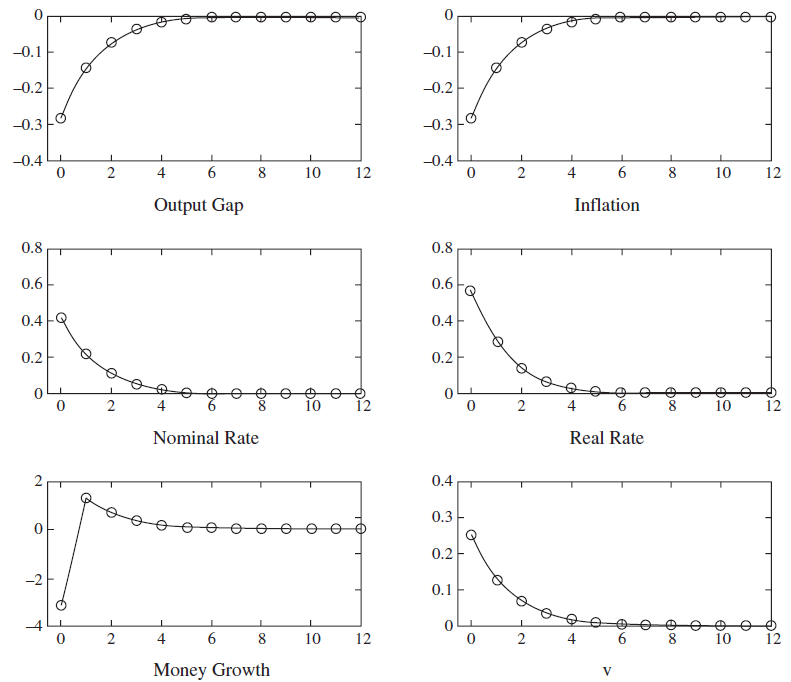
\includegraphics[width=0.65\textwidth]{FIGURES/11_Gali_Fig3_1}
%	%\subfigure{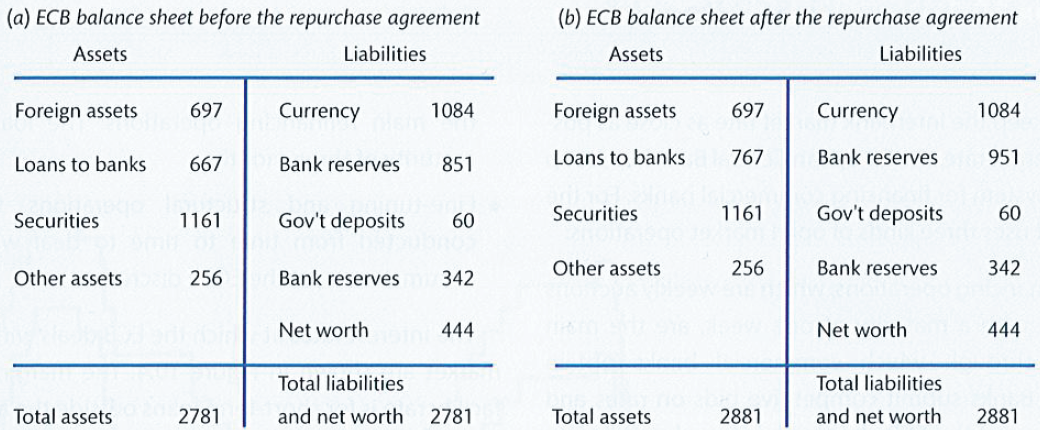
\includegraphics[trim=0 00 0 00,clip,width=0.6\textwidth]{FIGURES/5_CB_balance_sheet_OMO}
%	%} 	
%	%[trim=left bottom right top
%\end{figure}
%\vspace{-0.2cm}
%\begin{minipage}{0.5\columnwidth}
%\tiny
%	
%\textbf{Source.} Gal\'{i} (2008), Figure 3.1.\\
%\end{minipage}
%\end{center}
%
%\end{frame}
%%---FRAME------------------------------------------------------------------------------
%\begin{frame}{Effect of monetary policy: empirical estimates}
%
%
%\begin{center}
%{\small
%Figure. VAR estimates of a monetary policy shock
%}
%\vspace{-.1cm}
%\begin{figure}[h!]
%	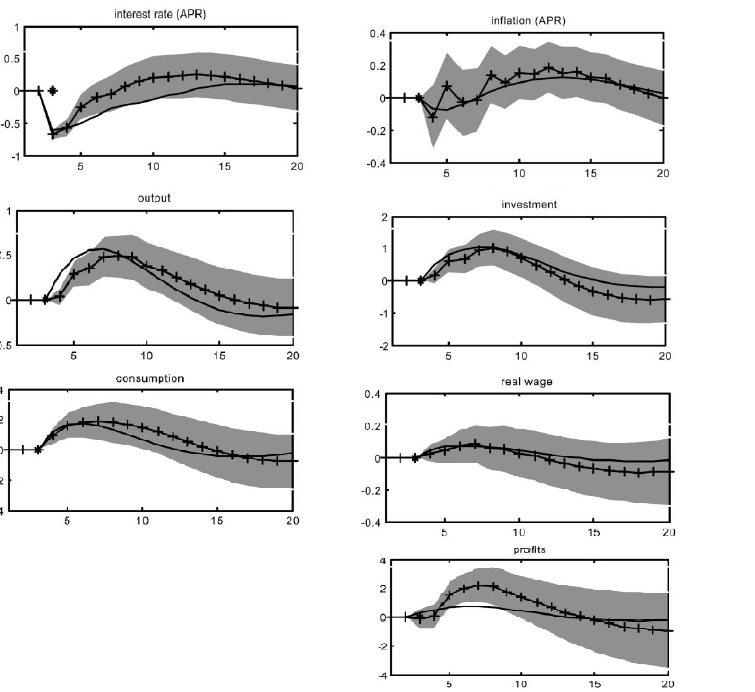
\includegraphics[width=0.65\textwidth]{FIGURES/CEE2005_IRFs}
%	%\subfigure{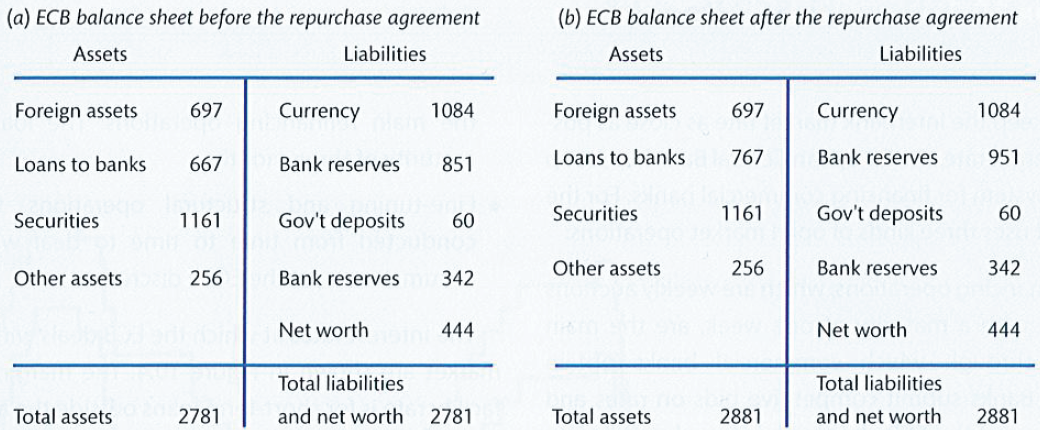
\includegraphics[trim=0 00 0 00,clip,width=0.6\textwidth]{FIGURES/5_CB_balance_sheet_OMO}
%	%} 	
%	%[trim=left bottom right top
%\end{figure}
%\vspace{-.2cm}
%\begin{minipage}{0.5\columnwidth}
%\tiny
%	
%\textbf{Note.} The impulse response to a \alert{expansionary} monetary policy shock \textbf{Source.} Christiano, Eichenbaum and Evans (2005), Figure 1.\\
%\end{minipage}
%\end{center}
%
%\end{frame}
%%---FRAME------------------------------------------------------------------------------
%\begin{frame}{Discussion (1) - quantitative results}
%
%{
%\small
%\begin{mytemize}
%\item Fit of the model \emph{qualitatively} okay, but quantitatively still room for improvements (e.g. no hump-shaped responses)
%\item propagation mechanism, however, reflected in the data
%\item Several modifications need to be implemented in order to better fit the data $\rightarrow$ medium scale DSGE models (Christiano, Eichenbaum \& Evans 2005, Smets \& Wouters 2003)
%\item such models can also be estimated (Lubik, Schorfheide 2005; Schorfheide 2007)
%\item \tb{NK model and policy}
%\begin{mytemize}
%\item the \emph{New Keynesian Phillips Curve} at center stage of policy making (e.g. role of inflation expectations, factors that affect the steepness of the PC,...). 
%%\item alternative models might lead to similar PC (Rothemberg 1982) or different PC (Mankiw \& Reis 2002)
%\item The \emph{natural rate hypothesis} underlying the baseline NK model heavily debated at the moment.
%%\item ($\rightarrow$\emph{topics in the TD presentations!})
%\end{mytemize}
%\end{mytemize}
%}
%
%\end{frame}
%%---FRAME------------------------------------------------------------------------------
%\begin{frame}{Discussion (2) - permanent effects of monetary policy?}
%
%Olivier Blanchard (JEP 2018) \\
%\emph{"Should We Reject the Natural Rate Hypothesis?"}
%\begin{mytemize}
%\item idea of \tb{hysteresis}
%\item effects that persist after initial cause
%\item leads to non-stationary time-series
%\begin{mytemize}
%\item labor markets (search and matching frictions)
%\item productivity (effect on R\&D)
%\end{mytemize}
%\end{mytemize}
%BUT: \\
%$\rightarrow$ Very persistent vs. permanent effects. \\
%$\rightarrow$ Empirical identification of causal effects close to impossible, but micro data can help.
%\end{frame}
%%---FRAME------------------------------------------------------------------------------
%\begin{frame}{Discussion (2) - permanent effects of monetary policy?}
%
%\begin{center}
%%{\small
%%Figure. 
%%}
%  \vspace{-.1cm}
%\begin{figure}[h!]
%	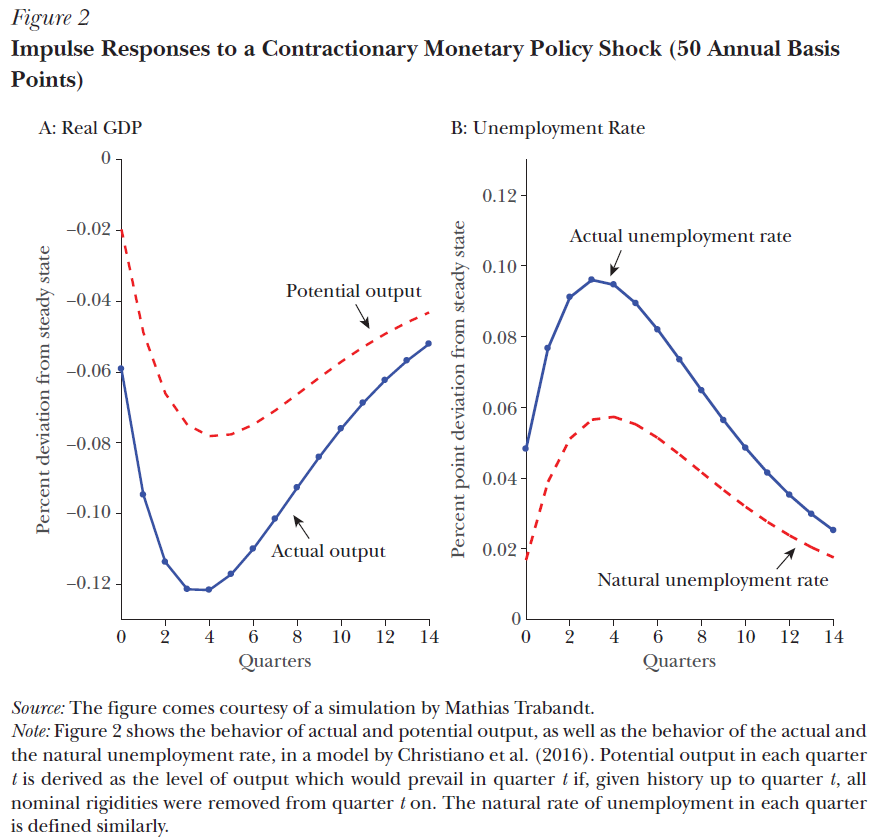
\includegraphics[width=0.85\textwidth]{FIGURES/Blanchard2018_MPeffectPotential}
%	%\subfigure{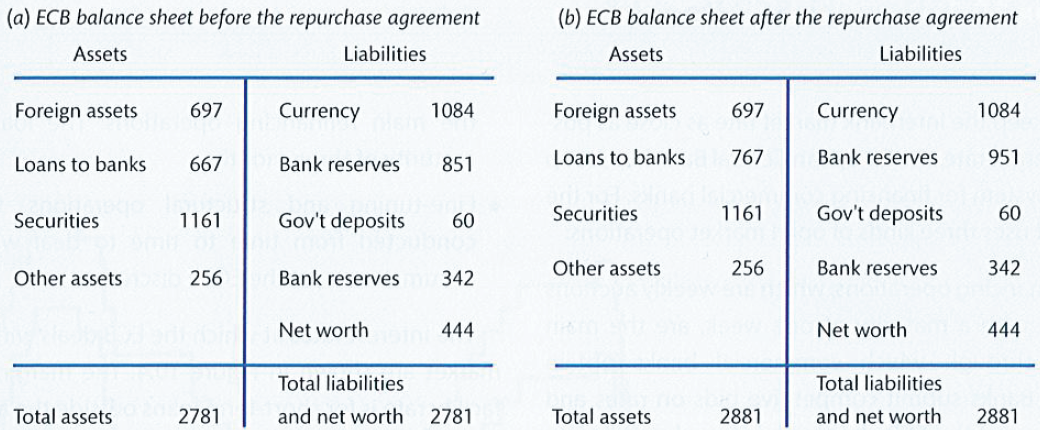
\includegraphics[trim=0 00 0 00,clip,width=0.6\textwidth]{FIGURES/5_CB_balance_sheet_OMO}
%	%} 	
%	%[trim=left bottom right top
%\end{figure}
%%\vspace{-2mm}
%%\begin{minipage}{0.5\columnwidth}
%%\tiny
%%	
%%\textbf{Note.} The impulse response to a \alert{expansionary} monetary policy shock \textbf{Source.} Christiano, Eichenbaum and Evans (2005), Figure 1.\\
%%\end{minipage}
%\end{center}
%
%\end{frame}
%%---FRAME------------------------------------------------------------------------------
%\begin{frame}{Discussion (2) - permanent effects of monetary policy?}
%
%{
%\small
% 
%\begin{center}
%%{\small
%%Figure. 
%%}
%  \vspace{-.1cm}
%\begin{figure}[h!]
%	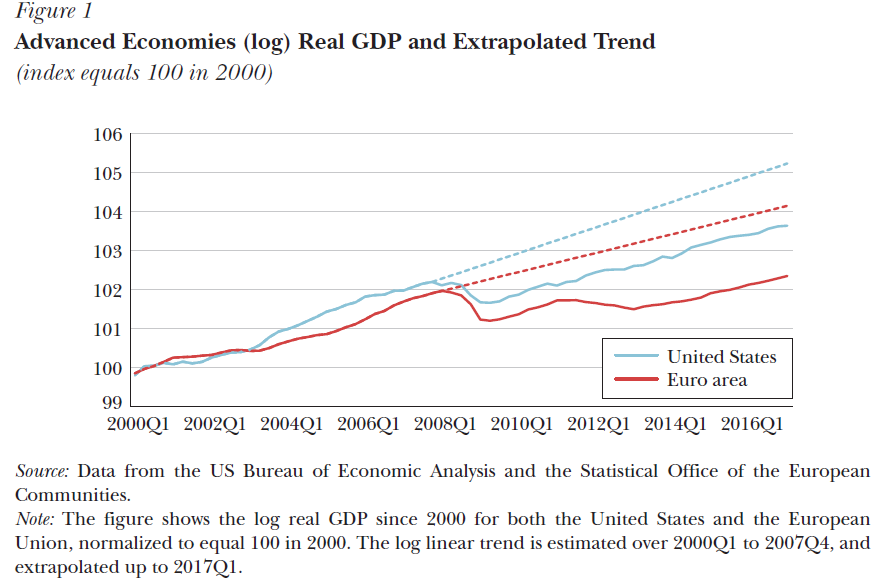
\includegraphics[width=0.95\textwidth]{FIGURES/Blanchard2018_GFC}
%	%\subfigure{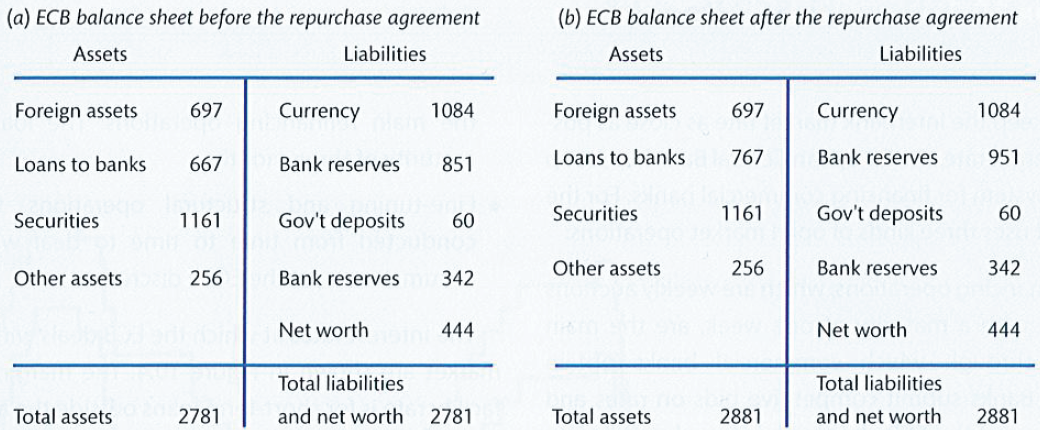
\includegraphics[trim=0 00 0 00,clip,width=0.6\textwidth]{FIGURES/5_CB_balance_sheet_OMO}
%	%} 	
%	%[trim=left bottom right top
%\end{figure}
%%\vspace{-2mm}
%%\begin{minipage}{0.5\columnwidth}
%%\tiny
%%	
%%\textbf{Note.} The impulse response to a \alert{expansionary} monetary policy shock \textbf{Source.} Christiano, Eichenbaum and Evans (2005), Figure 1.\\
%%\end{minipage}
%\end{center}
%
%}
%
%\end{frame}
%---FRAME------------------------------------------------------------------------------
%\section{The basic New Keynesian model}
%---FRAME------------------------------------------------------------------------------
%\begin{frame}
%\frametitle{Outline}
%\tableofcontents[currentsection]
%\end{frame}
%---FRAME------------------------------------------------------------------------------
%\begin{frame}{The basic New Keynesian model}

%\begin{mytemize}
%\small
%\item 
%\end{mytemize}

%\end{frame}
%---FRAME------------------------------------------------------------------------------
%\begin{frame}{Summary of the basic New Keynesian model}
%\begin{mytemize}
%\small
%\item see Burda Wyplosz p. 550
%\end{mytemize}
%\end{frame}
%---FRAME------------------------------------------------------------------------------
%\section{The Smets-Wouters model}
%---FRAME------------------------------------------------------------------------------
%\begin{frame}
%\frametitle{Outline}
%\tableofcontents[currentsection]
%\end{frame}
%---FRAME------------------------------------------------------------------------------
\end{document}

